
%% bare_conf.tex
%% V1.3
%% 2007/01/11
%% by Michael Shell
%% See:
%% http://www.michaelshell.org/
%% for current contact information.
%%
%% This is a skeleton file demonstrating the use of IEEEtran.cls
%% (requires IEEEtran.cls version 1.7 or later) with an IEEE conference paper.
%%
%% Support sites:
%% http://www.michaelshell.org/tex/ieeetran/
%% http://www.ctan.org/tex-archive/macros/latex/contrib/IEEEtran/
%% and
%% http://www.ieee.org/

%%*************************************************************************
%% Legal Notice:
%% This code is offered as-is without any warranty either expressed or
%% implied; without even the implied warranty of MERCHANTABILITY or
%% FITNESS FOR A PARTICULAR PURPOSE! 
%% User assumes all risk.
%% In no event shall IEEE or any contributor to this code be liable for
%% any damages or losses, including, but not limited to, incidental,
%% consequential, or any other damages, resulting from the use or misuse
%% of any information contained here.
%%
%% All comments are the opinions of their respective authors and are not
%% necessarily endorsed by the IEEE.
%%
%% This work is distributed under the LaTeX Project Public License (LPPL)
%% ( http://www.latex-project.org/ ) version 1.3, and may be freely used,
%% distributed and modified. A copy of the LPPL, version 1.3, is included
%% in the base LaTeX documentation of all distributions of LaTeX released
%% 2003/12/01 or later.
%% Retain all contribution notices and credits.
%% ** Modified files should be clearly indicated as such, including  **
%% ** renaming them and changing author support contact information. **
%%
%% File list of work: IEEEtran.cls, IEEEtran_HOWTO.pdf, bare_adv.tex,
%%                    bare_conf.tex, bare_jrnl.tex, bare_jrnl_compsoc.tex
%%*************************************************************************

% *** Authors should verify (and, if needed, correct) their LaTeX system  ***
% *** with the testflow diagnostic prior to trusting their LaTeX platform ***
% *** with production work. IEEE's font choices can trigger bugs that do  ***
% *** not appear when using other class files.                            ***
% The testflow support page is at:
% http://www.michaelshell.org/tex/testflow/



% Note that the a4paper option is mainly intended so that authors in
% countries using A4 can easily print to A4 and see how their papers will
% look in print - the typesetting of the document will not typically be
% affected with changes in paper size (but the bottom and side margins will).
% Use the testflow package mentioned above to verify correct handling of
% both paper sizes by the user's LaTeX system.
%
% Also note that the "draftcls" or "draftclsnofoot", not "draft", option
% should be used if it is desired that the figures are to be displayed in
% draft mode.
%
\documentclass[10pt,journal,letterpaper,compsoc]{IEEEtran}
% Add the compsocconf option for Computer Society conferences.
% 
% If IEEEtran.cls has not been installed into the LaTeX system files,
% manually specify the path to it like:
% \documentclass[conference]{../sty/IEEEtran}





% Some very useful LaTeX packages include:
% (uncomment the ones you want to load)


% *** MISC UTILITY PACKAGES ***
%
\usepackage{ifpdf}
% Heiko Oberdiek's ifpdf.sty is very useful if you need conditional
% compilation based on whether the output is pdf or dvi.
% usage:
% \ifpdf
%   % pdf code
% \else
%   % dvi code
% \fi
% The latest version of ifpdf.sty can be obtained from:
% http://www.ctan.org/tex-archive/macros/latex/contrib/oberdiek/
% Also, note that IEEEtran.cls V1.7 and later provides a builtin
% \ifCLASSINFOpdf conditional that works the same way.
% When switching from latex to pdflatex and vice-versa, the compiler may
% have to be run twice to clear warning/error messages.






% *** CITATION PACKAGES ***
%
%\usepackage{cite}
% cite.sty was written by Donald Arseneau
% V1.6 and later of IEEEtran pre-defines the format of the cite.sty package
% \cite{} output to follow that of IEEE. Loading the cite package will
% result in citation numbers being automatically sorted and properly
% "compressed/ranged". e.g., [1], [9], [2], [7], [5], [6] without using
% cite.sty will become [1], [2], [5]--[7], [9] using cite.sty. cite.sty's
% \cite will automatically add leading space, if needed. Use cite.sty's
% noadjust option (cite.sty V3.8 and later) if you want to turn this off.
% cite.sty is already installed on most LaTeX systems. Be sure and use
% version 4.0 (2003-05-27) and later if using hyperref.sty. cite.sty does
% not currently provide for hyperlinked citations.
% The latest version can be obtained at:
% http://www.ctan.org/tex-archive/macros/latex/contrib/cite/
% The documentation is contained in the cite.sty file itself.






% *** GRAPHICS RELATED PACKAGES ***
%
\ifCLASSINFOpdf
  % \usepackage[pdftex]{graphicx}
  % declare the path(s) where your graphic files are
  % \graphicspath{{../pdf/}{../jpeg/}}
  % and their extensions so you won't have to specify these with
  % every instance of \includegraphics
  % \DeclareGraphicsExtensions{.pdf,.jpeg,.png}
\else
  % or other class option (dvipsone, dvipdf, if not using dvips). graphicx
  % will default to the driver specified in the system graphics.cfg if no
  % driver is specified.
  % \usepackage[dvips]{graphicx}
  % declare the path(s) where your graphic files are
  % \graphicspath{{../eps/}}
  % and their extensions so you won't have to specify these with
  % every instance of \includegraphics
  % \DeclareGraphicsExtensions{.eps}
\fi
% graphicx was written by David Carlisle and Sebastian Rahtz. It is
% required if you want graphics, photos, etc. graphicx.sty is already
% installed on most LaTeX systems. The latest version and documentation can
% be obtained at: 
% http://www.ctan.org/tex-archive/macros/latex/required/graphics/
% Another good source of documentation is "Using Imported Graphics in
% LaTeX2e" by Keith Reckdahl which can be found as epslatex.ps or
% epslatex.pdf at: http://www.ctan.org/tex-archive/info/
%
% latex, and pdflatex in dvi mode, support graphics in encapsulated
% postscript (.eps) format. pdflatex in pdf mode supports graphics
% in .pdf, .jpeg, .png and .mps (metapost) formats. Users should ensure
% that all non-photo figures use a vector format (.eps, .pdf, .mps) and
% not a bitmapped formats (.jpeg, .png). IEEE frowns on bitmapped formats
% which can result in "jaggedy"/blurry rendering of lines and letters as
% well as large increases in file sizes.
%
% You can find documentation about the pdfTeX application at:
% http://www.tug.org/applications/pdftex





% *** MATH PACKAGES ***
%
%\usepackage[cmex10]{amsmath}
% A popular package from the American Mathematical Society that provides
% many useful and powerful commands for dealing with mathematics. If using
% it, be sure to load this package with the cmex10 option to ensure that
% only type 1 fonts will utilized at all point sizes. Without this option,
% it is possible that some math symbols, particularly those within
% footnotes, will be rendered in bitmap form which will result in a
% document that can not be IEEE Xplore compliant!
%
% Also, note that the amsmath package sets \interdisplaylinepenalty to 10000
% thus preventing page breaks from occurring within multiline equations. Use:
%\interdisplaylinepenalty=2500
% after loading amsmath to restore such page breaks as IEEEtran.cls normally
% does. amsmath.sty is already installed on most LaTeX systems. The latest
% version and documentation can be obtained at:
% http://www.ctan.org/tex-archive/macros/latex/required/amslatex/math/





% *** SPECIALIZED LIST PACKAGES ***
%
%\usepackage{algorithmic}
% algorithmic.sty was written by Peter Williams and Rogerio Brito.
% This package provides an algorithmic environment fo describing algorithms.
% You can use the algorithmic environment in-text or within a figure
% environment to provide for a floating algorithm. Do NOT use the algorithm
% floating environment provided by algorithm.sty (by the same authors) or
% algorithm2e.sty (by Christophe Fiorio) as IEEE does not use dedicated
% algorithm float types and packages that provide these will not provide
% correct IEEE style captions. The latest version and documentation of
% algorithmic.sty can be obtained at:
% http://www.ctan.org/tex-archive/macros/latex/contrib/algorithms/
% There is also a support site at:
% http://algorithms.berlios.de/index.html
% Also of interest may be the (relatively newer and more customizable)
% algorithmicx.sty package by Szasz Janos:
% http://www.ctan.org/tex-archive/macros/latex/contrib/algorithmicx/




% *** ALIGNMENT PACKAGES ***
%
%\usepackage{array}
% Frank Mittelbach's and David Carlisle's array.sty patches and improves
% the standard LaTeX2e array and tabular environments to provide better
% appearance and additional user controls. As the default LaTeX2e table
% generation code is lacking to the point of almost being broken with
% respect to the quality of the end results, all users are strongly
% advised to use an enhanced (at the very least that provided by array.sty)
% set of table tools. array.sty is already installed on most systems. The
% latest version and documentation can be obtained at:
% http://www.ctan.org/tex-archive/macros/latex/required/tools/


%\usepackage{mdwmath}
%\usepackage{mdwtab}
% Also highly recommended is Mark Wooding's extremely powerful MDW tools,
% especially mdwmath.sty and mdwtab.sty which are used to format equations
% and tables, respectively. The MDWtools set is already installed on most
% LaTeX systems. The lastest version and documentation is available at:
% http://www.ctan.org/tex-archive/macros/latex/contrib/mdwtools/


% IEEEtran contains the IEEEeqnarray family of commands that can be used to
% generate multiline equations as well as matrices, tables, etc., of high
% quality.


%\usepackage{eqparbox}
% Also of notable interest is Scott Pakin's eqparbox package for creating
% (automatically sized) equal width boxes - aka "natural width parboxes".
% Available at:
% http://www.ctan.org/tex-archive/macros/latex/contrib/eqparbox/





% *** SUBFIGURE PACKAGES ***
%\usepackage[tight,footnotesize]{subfigure}
% subfigure.sty was written by Steven Douglas Cochran. This package makes it
% easy to put subfigures in your figures. e.g., "Figure 1a and 1b". For IEEE
% work, it is a good idea to load it with the tight package option to reduce
% the amount of white space around the subfigures. subfigure.sty is already
% installed on most LaTeX systems. The latest version and documentation can
% be obtained at:
% http://www.ctan.org/tex-archive/obsolete/macros/latex/contrib/subfigure/
% subfigure.sty has been superceeded by subfig.sty.



%\usepackage[caption=false]{caption}
%\usepackage[font=footnotesize]{subfig}
% subfig.sty, also written by Steven Douglas Cochran, is the modern
% replacement for subfigure.sty. However, subfig.sty requires and
% automatically loads Axel Sommerfeldt's caption.sty which will override
% IEEEtran.cls handling of captions and this will result in nonIEEE style
% figure/table captions. To prevent this problem, be sure and preload
% caption.sty with its "caption=false" package option. This is will preserve
% IEEEtran.cls handing of captions. Version 1.3 (2005/06/28) and later 
% (recommended due to many improvements over 1.2) of subfig.sty supports
% the caption=false option directly:
%\usepackage[caption=false,font=footnotesize]{subfig}
%
% The latest version and documentation can be obtained at:
% http://www.ctan.org/tex-archive/macros/latex/contrib/subfig/
% The latest version and documentation of caption.sty can be obtained at:
% http://www.ctan.org/tex-archive/macros/latex/contrib/caption/




% *** FLOAT PACKAGES ***
%
%\usepackage{fixltx2e}
% fixltx2e, the successor to the earlier fix2col.sty, was written by
% Frank Mittelbach and David Carlisle. This package corrects a few problems
% in the LaTeX2e kernel, the most notable of which is that in current
% LaTeX2e releases, the ordering of single and double column floats is not
% guaranteed to be preserved. Thus, an unpatched LaTeX2e can allow a
% single column figure to be placed prior to an earlier double column
% figure. The latest version and documentation can be found at:
% http://www.ctan.org/tex-archive/macros/latex/base/



%\usepackage{stfloats}
% stfloats.sty was written by Sigitas Tolusis. This package gives LaTeX2e
% the ability to do double column floats at the bottom of the page as well
% as the top. (e.g., "\begin{figure*}[!b]" is not normally possible in
% LaTeX2e). It also provides a command:
%\fnbelowfloat
% to enable the placement of footnotes below bottom floats (the standard
% LaTeX2e kernel puts them above bottom floats). This is an invasive package
% which rewrites many portions of the LaTeX2e float routines. It may not work
% with other packages that modify the LaTeX2e float routines. The latest
% version and documentation can be obtained at:
% http://www.ctan.org/tex-archive/macros/latex/contrib/sttools/
% Documentation is contained in the stfloats.sty comments as well as in the
% presfull.pdf file. Do not use the stfloats baselinefloat ability as IEEE
% does not allow \baselineskip to stretch. Authors submitting work to the
% IEEE should note that IEEE rarely uses double column equations and
% that authors should try to avoid such use. Do not be tempted to use the
% cuted.sty or midfloat.sty packages (also by Sigitas Tolusis) as IEEE does
% not format its papers in such ways.





% *** PDF, URL AND HYPERLINK PACKAGES ***
%
%\usepackage{url}
% url.sty was written by Donald Arseneau. It provides better support for
% handling and breaking URLs. url.sty is already installed on most LaTeX
% systems. The latest version can be obtained at:
% http://www.ctan.org/tex-archive/macros/latex/contrib/misc/
% Read the url.sty source comments for usage information. Basically,
% \url{my_url_here}.


%my own packages
\usepackage{verbatim}
\usepackage{epsfig}
\usepackage{paralist}
\usepackage{algorithmic}
\usepackage{algorithm}
\usepackage{url}

%my own environment variables
\newtheorem{claim}{Claim}
\newtheorem{lemma}{Lemma}
\newtheorem{corollary}[lemma]{Corollary}
\newtheorem{definition}{Definition}
\newtheorem{observation}{Observation}
\newtheorem{constraint}{Constraint}

\def\colrule{\\[-7pt]\hline\\[-6pt]}


\makeatletter
\def\imod#1{\allowbreak\mkern10mu({\operator@font mod}\,\,#1)}
\makeatother
% *** Do not adjust lengths that control margins, column widths, etc. ***
% *** Do not use packages that alter fonts (such as pslatex).         ***
% There should be no need to do such things with IEEEtran.cls V1.6 and later.
% (Unless specifically asked to do so by the journal or conference you plan
% to submit to, of course. )


% correct bad hyphenation here
\hyphenation{op-tical net-works semi-conduc-tor}


\begin{document}


%
% paper title
% can use linebreaks \\ within to get better formatting as desired
\title{
%Improving the scalability of protein sequence clustering for large-scale metagenomic data sets
{\it pGraph}: Efficient Parallel Construction of Large-Scale Protein Sequence Homology Graphs 
}


% author names and affiliations
% use a multiple column layout for up to two different
% affiliations
\author{Changjun Wu,
        Ananth Kalyanaraman,
        and William R. Cannon% <-this % stops a space
\IEEEcompsocitemizethanks{\IEEEcompsocthanksitem C. Wu and A. Kalyanaraman are with the School of Electrical Engineering and Computer Science, Washington State University, Pullman, WA, 99164.\protect\\
% note need leading \protect in front of \\ to get a newline within \thanks as
% \\ is fragile and will error, could use \hfil\break instead.
E-mail: \{cwu2, ananth\}@eecs.wsu.edu
\IEEEcompsocthanksitem W.R. Cannon is with Pacific Northwest National Laboratory, Richland, WA. 99352.\protect\\
E-mail: william.cannon@pnl.gov}
\thanks{}}

% conference papers do not typically use \thanks and this command
% is locked out in conference mode. If really needed, such as for
% the acknowledgment of grants, issue a \IEEEoverridecommandlockouts
% after \documentclass

% for over three affiliations, or if they all won't fit within the width
% of the page, use this alternative format:
% 
%\author{\IEEEauthorblockN{Michael Shell\IEEEauthorrefmark{1},
%Homer Simpson\IEEEauthorrefmark{2},
%James Kirk\IEEEauthorrefmark{3}, 
%Montgomery Scott\IEEEauthorrefmark{3} and
%Eldon Tyrell\IEEEauthorrefmark{4}}
%\IEEEauthorblockA{\IEEEauthorrefmark{1}School of Electrical and Computer Engineering\\
%Georgia Institute of Technology,
%Atlanta, Georgia 30332--0250\\ Email: see http://www.michaelshell.org/contact.html}
%\IEEEauthorblockA{\IEEEauthorrefmark{2}Twentieth Century Fox, Springfield, USA\\
%Email: homer@thesimpsons.com}
%\IEEEauthorblockA{\IEEEauthorrefmark{3}Starfleet Academy, San Francisco, California 96678-2391\\
%Telephone: (800) 555--1212, Fax: (888) 555--1212}
%\IEEEauthorblockA{\IEEEauthorrefmark{4}Tyrell Inc., 123 Replicant Street, Los Angeles, California 90210--4321}}




% use for special paper notices
%\IEEEspecialpapernotice{(Invited Paper)}

% for Computer Society papers, we must declare the abstract and index terms
% PRIOR to the title within the \IEEEcompsoctitleabstractindextext IEEEtran
% command as these need to go into the title area created by \maketitle.
\IEEEcompsoctitleabstractindextext{%
\begin{abstract}
%\boldmath
Detecting sequence homology between protein sequences is a fundamental problem in computational molecular biology, with a pervasive application in nearly all analyses that aim to structurally and functionally characterize protein molecules. While detecting the homology between two protein sequences is relatively inexpensive, detecting pairwise homology for a large number of protein sequences can become computationally prohibitive for modern inputs, often requiring millions of CPU hours. Yet, there is currently no robust support to parallelize this kernel. In this paper, we identify the key characteristics that make this problem particularly hard to parallelize, and then propose a new parallel algorithm that is suited for detecting homology on large data sets using distributed memory parallel computers. Our method, called {\it pGraph}, is a novel hybrid between the hierarchical multiple-master/worker model and producer-consumer model, and is designed to break the irregularities imposed by alignment computation and work generation. Experimental results show that {\it pGraph} achieves linear scaling on a 2,048 processor distributed memory cluster for a wide range of inputs ranging from as small as 20,000 sequences to 2,560,000 sequences. In addition to demonstrating strong scaling, we present an extensive report on the performance of the various system components and related parametric studies. 
\end{abstract}
% IEEEtran.cls defaults to using nonbold math in the Abstract.
% This preserves the distinction between vectors and scalars. However,
% if the journal you are submitting to favors bold math in the abstract,
% then you can use LaTeX's standard command \boldmath at the very start
% of the abstract to achieve this. Many IEEE journals frown on math
% in the abstract anyway. In particular, the Computer Society does
% not want either math or citations to appear in the abstract.

% Note that keywords are not normally used for peer review papers.
\begin{keywords}
Parallel protein sequence homology detection; parallel sequence graph construction; hierarchical master-worker paradigm, producer-consumer model.
\end{keywords}}


% make the title area
\maketitle

% For peer review papers, you can put extra information on the cover
% page as needed:
% \ifCLASSOPTIONpeerreview
% \begin{center} \bfseries EDICS Category: 3-BBND \end{center}
% \fi
%
% For peerreview papers, this IEEEtran command inserts a page break and
% creates the second title. It will be ignored for other modes.
\IEEEpeerreviewmaketitle

\section{Introduction}
\label{secIntroduction}

Protein sequence homology detection is a fundamental problem in computational molecular biology. Given a set of protein sequences, the goal is to identify all highly ``similar'' pairs of sequences, where similarity constraints are typically defined using an alignment model (e.g., \cite{Needleman70,Smith81}). In graph-theoretic terms, the protein sequence homology detection problem can be thought of as constructing an undirected graph $G(V,E)$, where $V$ is the set of input protein sequences and $E$ is the set of edges $(v_i,v_j)$ such that the sequences corresponding to $v_i$ and $v_j$ are highly similar.

Homology detection is widely used in nearly all analyses targeted at functional and structural characterization of protein molecules \cite{Kriventseva01}. Most notably, it is used as a precursor step to clustering, which aims at partitioning sequences into closely-knit groups of functionally and/or structurally related proteins called ``families''. In graph-theoretic terms, this is equivalent of finding variable-sized maximal cliques. However, in practice, owing to errors in sequence data and other biological considerations (e.g., functionally related proteins could differ at the sequence level), the problem becomes one of finding densely connected subgraphs \cite{Olman07,Wu08,Yooseph07}. Protein sequence clustering is gaining importance of late because of its potential to uncover and functionally annotate environmental microbial communities (aka.  metagenomic data) \cite{Handelsman04}. For instance, a single study in 2007 that surveyed an ocean microbiota \cite{Yooseph07} resulted in the discovery of nearly $4\times 10^3$ previously unknown protein families, significantly expanding the protein universe as we know it. %Homology detection and clustering play a central role during family identification. 

While there are a number of programs available for protein sequence clustering (e.g., \cite{Apweiler04,Bateman04,Enright02,Kriventseva01,Olman07}), all of them assume that the graph can be easily built or is readily available as input. However, modern-day use-cases suggest otherwise. Large-scale projects generate millions of \emph{new} sequences that need to be matched against themselves and against sequences already available from previous sequencing projects. For example, the ocean metagenomic project generated more than 17 million new sequences and this set was analyzed alongside 11 million sequences in public protein sequence databanks (for a total of 28.6 million sequences). Consequently, the most time consuming step during analysis was homology detection, which alone accounted for $10^6$ CPU hours despite the use of faster approximation heuristics such as BLAST \cite{Altschul90} to determine homology. Ideally, dynamic programming algorithms \cite{Needleman70,Smith81} that guarantee alignment optimality should be the method of choice as they are generally more sensitive but the associated high cost of computation coupled with a lack of support in software for coarse-level parallelism have impeded their application under large-scale settings.

In this paper, we address the problem of parallelizing homology graph construction on massive protein sequence data sets, and one that will enable the deployment of the optimality-guaranteeing dynamic programming algorithms as the basis for pairwise homology detection (or equivalently, edge detection). Although at the offset the problem may appear embarrassingly parallel (because the evaluation of each edge is an independent task), several practical considerations and our own experience \cite{Wu08} suggest it is a non-trivial problem.

Firstly, the problem is data-intensive, even more so than its DNA counterpart. While the known protein universe is relatively small, modern use-cases particularly in metagenomics, in an attempt to find new proteins and families, generate millions of DNA sequences first and then convert them into amino acid sequences corresponding to all six reading frames as protein candidates for evaluation, resulting in a 6$\times$ increase in data volume for analysis\footnote{Henceforth for simplicity of exposition, we will use the terms ``amino acid sequences'' and ``protein sequences'' interchangeably; although in practice an amino acid sequence need not represent a complete or real protein sequence.}. Tens of millions of such amino acid sequences are already available from public repositories (e.g., CAMERA \cite{CAMERA}, IMG/M \cite{IMG08} ). Large data size creates two complications.  
\begin{compactenum}[i)]
\item
 A brute-force all-against-all sequence comparison strategy to detect the presence of edges becomes practically unfeasible due to the quadratic explosion of alignment work. Instead, a filtering based strategy, one that short-lists a smaller subset of sequence pairs based on their potential to pass the alignment criteria prior to actually computing the alignments, needs to be used. In practice, exact matching filters that deploy string data structures such as suffix trees \cite{Weiner73} are highly effective in reducing alignment work without compromising on quality \cite{KalyanaramanNAR03,KalyanaramanJPDC07}. While the time consumed by these advanced filters for pair generation is relatively less when compared to alignment computation, it is certainly \emph{not negligible}. From a parallel implementation standpoint, this means that we could not use a standard work distribution tool --- in order to take advantage of these effective sophisticated filters, work generation also needs to be parallelized dynamically alongside work processing. 
\item
A large data size also means that the local availability of sequences during alignment processing cannot be guaranteed under the distributed memory machine setting. Alternatively, moving computation to data is also virtually impossible because a pair identified for alignment work could involve arbitrary sequences and could appear in an arbitrary order during generation, both of which are totally data-dependent. 
\end{compactenum}

Secondly, handling amino acid sequence data gives rise to some unique \emph{irregularity} issues that need to be contended with during parallelization. i) Assuming ``work'' refers to a pair of sequences designated for alignment computation, \emph{the time to process each unit of work could be highly variable}. This is because the time for aligning two sequences using dynamic programming takes time proportional to the product of the lengths of the two sequences \cite{Needleman70,Smith81}. And, amino acid sequences tend to have a substantial variability in their lengths, as we will also shown in Section~\ref{secResults}. 
ii) For amino acid data, \emph{the rate at which work is generated could also be non-uniform}. For instance, similar sized portions of the suffix tree index could yield drastically different number of sequence pairs, as the composition of the index is data dependent. {\it A priori} stocking of pairs that require alignment is simply not an option because of a worst-case quadratic requirement.

Note that these challenges do not typically arise when dealing with DNA. For instance, in genome sequencing projects the lengths of raw DNA sequences derived from modern day DNA sequencers are typically uniform. This coupled with the nature of sampling typically leads to predictable work during generation and processing. In case of metagenomics protein data, the higher variability in sequence lengths is a result of the translation done on the assembled products of DNA assembly (i.e., not raw DNA sequences). Because of this variability, analysis of protein data tends to take longer time and more difficult to parallelize. For example, in the human genome assembly project \cite{Venter01}, the all-against-all sequence homology detection of roughly 28 million DNA sequences consumed only $10^4$ CPU hours. Contrast this with the $10^6$ CPU hours observed for analyzing roughly the same number of protein sequences in the ocean metagenomic project despite the use of much faster hardware \cite{Yooseph07}.


\subsection{Contributions}
\label{secContributions}


In this paper, we present a new algorithm to carry out large-scale protein sequence homology detection. Our algorithm, called {\it pGraph}\footnote{stands for ``\underline{p}arallel construction of protein sequence homology \underline{Graph}''}, is designed to take advantage of the large-scale memory and compute power available from distributed memory parallel machines. The output is the set of edges in the sequence homology graph which can be readily used as input for subsequent post-processing steps such as clustering. 

Our parallel approach represents a hybrid variant between hierarchical multiple-master/worker and producer-consumer models. The processor space is organized into fixed-size subgroups; each subgroup comprising of possibly multiple ``producers'' (for pair generation), a local master (for local pair distribution) and a fixed number of ``consumers'' (for alignment computation). A dedicated global master (``supermaster'') manages the workload across subgroups through dynamic load balancing and task reallocation across the subgroups. The producer-consumer division, inspired by the Map Reduce parallel paradigm \cite{Dean08}, helps decouple the two major operations in the code, while also providing the flexibility and user-level control to configure the system resources as per input demands. These techniques combined with other base principles in parallel program design for distributed memory computers have allowed us to accommodate the use of quality-enhancing dynamic programming algorithms for evaluating alignments and determining homology at a massive scale. 

Experimental results show that {\it pGraph} achieves linear scaling on a 2,048 processor distributed memory cluster for a wide range of inputs ranging from as small as 20,000 sequences to 2,560,000 sequences. Furthermore, the implementation is able to maintain more than 90\% parallel efficiency despite the considerable volume of data movement and the dedication of resources to the hierarchy. In addition to these strong scaling results, we present a thorough anatomical study of the system-wide behavior by its different components. We also comparatively evaluate two models of our algorithm, one that uses I/O and another that uses interprocess communication, for fetching sequences required for alignment computation. 

Though presented in the context of protein sequence graph construction, we expect that the basic design principles of our approach can extend to other similar data-intensive scientific applications that involve an element of irregularity or unpredictability concerning work generation, work processing and input data movement.
The paper is organized as follows. Section~\ref{secRelatedWork} presents the current state of art for parallel sequence homology detection. Section~\ref{secMethods} presents our proposed method and implementation details. Experimental results are presented and discussed in Section~\ref{secResults}, and Section~\ref{secConclusions} concludes the paper.

%The highlights of the parallel design are as follows: The method uses a hierarchical multiple-master multiple-worker model to dynamically distribute tasks corresponding to both work generation and work processing in a load balanced fashion. The processor space is organized into subgroups with each subgroup comprising of possibly multiple ``producers'' (for work generation), a local master (for work distribution) and a fixed number of workers acting as ``consumers'' of work. This producer-consumer model of organizing processors helps decouple work generation from work processing. In addition, a dedicated global master (``supermaster'') is tasked with the responsibility of managing the workload across subgroups. Each node stores only a portion of the input set of sequences. We implemented and tested two versions, one that uses I/O and another that uses interprocess communication, for sequence fetches during alignment computation.


\section{Background and Related Work}
\label{secRelatedWork}

Sequence homology between two biomolecular sequences can be evaluated either using rigorous optimal alignment algorithms in time proportional to product of the sequence lengths \cite{Needleman70,Smith81}, or using faster, approximation heuristic methods such as BLAST \cite{Altschul90} and FASTA \cite{Pearson88}. Detecting the presence or absence of pairwise homology for a \emph{set} of protein/amino acid sequences, which is the subject of this article, can be modeled as a homology graph construction problem with numerous applications (e.g., \cite{Apweiler04,Bateman04,Enright02,Kriventseva01,Olman07}). The rapid adoption of cost-effective, high throughput sequencing technologies is contributing  millions of new sequences  into sequence repositories \cite{CAMERA,IMG08,NCBI}. As a result, detection of pairwise homology over these large data sets is becoming a daunting computational task. 

An indirect option for implementing homology detection is to use the BLAST program \cite{Altschul90}, which is a method originally designed for performing sequence database search (query vs. database). This can be done by setting both the query and database sets to the input set of sequences. For instance, the ocean metagenomics survey project \cite{Yooseph07} used BLAST to perform all-against-all sequence comparison. This took $10^6$ CPU hours --- a task that was parallelized, albeit in an {\it ad hoc} manner, by manually partitioning across 125 dual processors systems and 128 16-processor nodes each containing between 16GB-64GB of RAM. Several parallel tools are available for BLAST --- the most notable tools being mpiBLAST \cite{Darling03} and ScalaBLAST \cite{Oehmen06}. These methods run the serial version of NCBI BLAST at their cores, while offering a high degree of coarse-level parallelism and have demonstrated scaling  to high-end parallel machines. In addition to being relatively quicker, BLAST also provides a statistical score of significance for comparing a query sequence against a database of sequences. 

The use of BLAST based techniques however comes with reduced sensitivity \cite{Pearson91,Shpaer96} as the underlying algorithm is really an approximation heuristic for computing alignments. Comparatively, the dynamic programming algorithms offer alignment optimality but are generally an order of magnitude slower. Nevertheless, sensitivity is becoming a significant concern of late, especially when dealing with metagenomics data processing because of its highly fragmented nature of sampling. Another less desirable side effect of using BLAST for protein sequence data is that it uses the lookup table data structure which is limited to detection of only short, fixed-length matches between pairs of sequences. This could result in more pairs to be evaluated. Other string data structures such as suffix trees provide more specificity when it comes to the choice of pairs to evaluate due to their ability to detect longer, variable-length matches. 

Due to the advantages in using dynamic programming, there has been a flurry of efforts for implementing hardware-level acceleration for optimal pairwise sequence alignment computation on different architectures (reviewed in \cite{Sarkar10}). However, there is a dearth in research that has targeted at achieving coarse-level parallelism for carrying out millions of such alignment computations. There have been a few efforts for DNA sequence analysis \cite{KalyanaramanTPDS03,KalyanaramanJPDC07}, but carrying out protein sequence homology detection at a large-scale has not been addressed to the best of our knowledge.


%These advantages are however offset by the fact that any BLAST based solution is really an approximation heuristic, while the use of dynamic programming algorithms guarantees alignment optimality. It has been shown that computing optimal alignments helps improve sensitivity to varying degrees in practice \cite{} and sensitivity is an ubiquitous challenge with metagenomics data processing (due to its high fragmented nature of sampling). 

The purpose of this paper is to investigate the development of a new parallel library that supports large-scale homology detection based on optimal alignment computation. As part of one of our earlier efforts to implement parallel protein clustering \cite{Wu08}, we implemented a master-worker framework for homology detection based on optimal alignment computation. Performance evaluation showed that the pairwise sequence homology detection phase, which accounted for more than 90\% of the total runtime, failed to scale linearly beyond 128 processors \cite{Wu08}. The cause for the slowdown was primarily the irregular rates at which pairs were generated and processed. Interestingly, the same scheme had demonstrated linear scaling on DNA sequence clustering problems earlier \cite{KalyanaramanTPDS03,KalyanaramanJPDC07}, corroborating the higher complexity in analyzing protein sequences.

While there are dynamic load balancing schemes in parallel processing to mitigate the effects of variability in work processing rates, such techniques have traditionally suited compute-intensive applications. The data-intensive characteristic of the homology detection application is additionally challenged with data movement and availability issues. Recently, the mpiBLAST team proposed a highly scalable hierarchical master-worker framework for parallelizing the sequence search operation of BLAST \cite{Lin10}. However, the challenges posed by this problem are different from ours. In addition to being a query-to-database search operation, the unpredictability in BLAST is a result of the variability in query processing times; some queries can take more time the others. On the other hand, the number of task units are predictable as each query sequence is compared against the entire database (i.e., against all its fragments). In our problem, these task units (i.e., pairs to be aligned) are also detemined dynamically and in no predictable order. This results in an explicit task-level separation between work generation (i.e., pair generation from the suffix tree index) and work processing (i.e., alignment), and variability could be expected in both phases.  This led us to investigate a different version of a hierarchical master-worker model and combine it with a producer-consumer model inspired by the Map Reduce paradigm.

\section{Methods}
\label{secMethods}

\noindent{\bf Notation:} Let $S=\{s_1,s_2,\ldots s_n\}$ denote the set of $n$ input protein sequences. Assuming $|s|$ denotes the length of sequence $s$ and $m=\Sigma_{i=1}^n |s_i|$ denotes the total length of all sequences in $S$. Let $G=(V,E)$ denote a graph defined as $V=S$ and $E=\{(s_i,s_j)$ $|$ $s_i$ and $s_j$ are ``similar'', defined as per pre-defined alignment cutoffs\}. We use the term ``pair'' in this paper to refer to an arbitrary pair of sequences $(s_i,s_j)$. \\

\noindent{\bf Problem statement:} Given a set $S$ of $n$ protein sequences and $p$ processors, the protein sequence graph construction problem is to detect and output the edges of $G$ in parallel.\\



%\begin{figure}[tb]
%\centerline{
						%\scalebox{0.7}{\input{figFramework.pstex_t}}
%						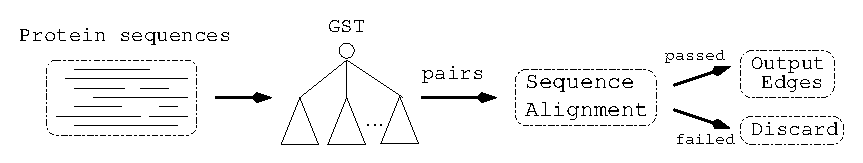
\includegraphics[angle=0, scale=0.60]{icppFram.eps}
%            }
%\caption{
%Tree-based filtering scheme used by our approach for protein sequence homology detection. $GST$ stands for Generalized %Suffix Tree.
%}
%\label{figFramework}
%\end{figure}

\subsection{Pair generation}
\label{secGeneratingPairs}

A brute-force approach to detect the presence of an edge is to enumerate all possible  pairs of sequences ($n\choose 2$) and retain only those as edges which pass the alignment test. Alternatively, since alignments represent approximate matching, the presence of long exact matches can be used as a necessary but not sufficient condition. This approach can filter out a significant fraction of poor quality pairs and thereby reduce the number of pairs to be aligned significantly. Suffix tree based filters provide one of the best filters --- for instance, anywhere between 67\% to over 99\% savings for our experiments shown later in the results section (Table~\ref{tabRuntime}). 


To implement exact matching using suffix trees, we use the optimal pair generation algorithm described in \cite{KalyanaramanTPDS03}, which detects and reports all pairs that share a maximal match of a minimum length $\psi$. The algorithm first builds a Generalized Suffix Tree (GST) data structure \cite{Weiner73} as a string index for the strings in $S$ and then traverses the tree in a bottom-up fashion to generate pairs from different nodes. Suffix tree construction is a well studied problem in both serial and parallel, and any of the standard, serial linear-time construction methods \cite{McCreight76,Ukkonen90,Weiner73} can be used, or efficient distributed memory codes can be used for parallelism \cite{KalyanaramanJPDC07,Ghoting09}.  Either way, the tree index can be generated in one preprocessing step and stored in the disk\footnote{Note that there are other, more space-efficient alternatives to suffix trees such as suffix arrays and enhanced suffix arrays, which can also be equivalently used to generate these pairs with some appropriate changes to the pair generation code. We omit those details from this article as pair generation is not the focus of this paper. That said the type of challenges dealt with the tree during parallel pair generation and the solutions proposed would still carry over to these other representations.}. 

For our purpose, we generate the tree index as a forest of disjoint subtrees emerging at a specified depth $\leq\psi$, so that the individual subtrees can be independently traversed in parallel to generate pairs. Given that the value of $\psi$ is typically a small user-specified constant, the choice for the cutting depth is restricted too. This implies that the size distribution of the resulting subtrees can be \emph{nonuniform} and is input dependent. It is also to be noted that, even though the pair generation algorithm runs in time bound by the number of output pairs, the process of generation itself could also be \emph{nonuniform} --- in that, subtrees of similar size could produce different number of pairs and/or at different rates, and the behavior is input-dependent. For instance, if a section of subtree receives a highly repetitive fraction of the input sequences then it is bound to generate a disproportionately large number of pairs. Encouragingly, a small value for the cutting depth is \emph{not} a limiting factor when it comes to the number of subtrees and is sufficient to support a high degree of parallelism. This is because the number of subtrees is expected to grow exponentially with the cutting depth; for instance, a cutting depth as small as 4 on a tree built out of protein sequences (alphabet size 20) could produce around $160K$ trees (as shown in experimental results). 


%\subsubsection{Computing an alignment}
%\label{secAlignments}

%A pair of sequences $(s_i,s_j)$ short-listed by the pair generation algorithm are evaluated using the Smith-Waterman algorithm. For scoring amino acid substitutions between the two protein sequences, our default implementation uses a user-specified substitution matrix such as BLOSUM62 \cite{Henikoff92}. For alignment criteria, we use the same parameters described in \cite{Wu08, Yooseph07}. If a pair passes this alignment test, then it is output as an edge into a file. Furthermore, an additional check is performed to see if one of the sequences in the pair is contained within the other sequence, and if so, it is marked as a ``redundant sequence'' and output to another file. 


\subsection{{\it pGraph}: Parallel graph construction}
\label{secMasterSlave}



\begin{figure*}[tb]
\centerline{
						\scalebox{0.8}{\input{figPClust.pstex_t}}
            }
\caption{
The overall system architecture for {\it pGraph}.
}
\label{figPClust}
\end{figure*}
\begin{comment}
ANDY: TO THE LEFT OF THE SUPERMASTER ADD A DISK LIKE PICTURE AND INSIDE THAT SHOW A FOREST OF SUBTREES.
\end{comment}

We present here an efficient parallel algorithm to construct the homology graph $G$ using the suffix tree index constructed in the previous step and the input sequence set $S$.  The inputs include the sequence set $S$ and the tree index $T$. The tree index is available as a forest of $k$ subtrees, which we denote as $T=\{t_1,t_2,\ldots t_k\}$.  The output of {\it pGraph} should be the set of all edges of the form $(s_i,s_j)$ s.t., the sequences $s_i$ and $s_j$ pass the alignment test based on user-defined cutoffs. There are two major operations that need to be performed in parallel: i) generate pairs from the tree index; and ii) compute sequence alignments and output edges if they pass the predefined cutoffs.

%and iii) output edges of the graph $G$ that satisfy an alignment cutoff. 

Our method uses a hybrid variant between the hierarchical multiple-master/worker model and producer-consumer model to counter the challenges posed by the irregularities in pair generation and alignment rates. The overall system architecture is illustrated in Figure~\ref{figPClust}. 

Given $p$ processors and a small number $q\geq 3$, the parallel system is partitioned as follows: i) one processor is designated to act as the \emph{supermaster} for the entire system; and ii) the remaining $p-1$ processors are partitioned into subgroups of size $q$ processors each\footnote{With the possible exception of the last subgroup which may obtain less than $q$ processors if $(p-1)\%q\ne 0$.}. Furthermore, each subgroup is internally organized with $r$ processors designated to the role of a \emph{producer}, one processor to the role of a \emph{master}, and $c$ processors to the role of a \emph{consumer}, where $c=q-r-1$. 

At a high level, the producers are responsible for pair generation, the masters for distributing the alignment workload within their respective subgroups, and the consumers for computing alignments. The supermaster plays a supervisory role to ensure load is distributed evenly among subgroups. Unlike traditional models, the overall data flow is from supermaster to the subgroups and also back (for redistribution). In what follows, we describe the various design factors and present algorithms and protocols for each component in the system. 

Let:\\
%\begin{itemize}\itemsep=-0.05ex
$P_{buf}\leftarrow$ a fixed sized pair buffer at the producer;\\
$M_{buf}\leftarrow$ a fixed sized pair buffer at the master;\\
$C_{buf}\leftarrow$ a fixed sized pair buffer at the consumer;\\
$S_{buf}\leftarrow$ a fixed sized pair buffer at the supermaster;\\
$b_1\leftarrow$ batch size (for pairs) from producer or supermaster to master;\\
$b_2\leftarrow$ batch size (for pairs) from master to consumer;\\


\subsubsection{Producer}
\label{secProducer}

The primary responsibility of a producer is to load a subset of subtrees in $T$ and generate pairs using the maximal matching algorithm in \cite{KalyanaramanTPDS03}. The main challenge here is that trees allocated at a producer could result in generation of pairs at a variable rate, although this generation rate is virtually guaranteed to be faster than the rate of consumption (alignment). This is because the pair generation is a simple cross product of sets at any given tree node. To tackle an overactive producer, we maintain a fixed-size pair buffer at each producer ($\sim 80MB$ in our current implementation) and pause the generation process when the buffer is full. This is possible because the pair generation algorithm in \cite{KalyanaramanTPDS03} is an on-demand method. Furthermore, the tree allocation is left to the supermaster and pair allocation from the producer is left to the local master in our design. 

More specifically,  we follow the algorithm shown in Algorithm~\ref{pd}. Initially, a producer fetches a batch of subtrees (available as a single file) from the supermaster. The producer then starts to generate and enqueue pairs into $P_{buf}$. Subsequently, the producer dequeues and sends $b_1$ pairs to the master. This is implemented using a nonblocking send so that when the master is not yet ready to accept pairs, the producer can continue to generate pairs, thereby allowing masking of communication. After processing the current batch of subtrees, the producer repeats the process by requesting another batch of subtrees from the supermaster. Once there are no more subtrees available, the producers dispatch the rest of pairs to both master \emph{and} supermaster, depending on whoever is responsive to their nonblocking sends. This strategy gives the producer an option of redistributing its pairs to other subgroups (via supermaster) if the local group is busy. We show in the experimental section that this strategy of using the supermaster route pays off significantly and ensures the system is load balanced. \\

\begin{algorithm}
\caption{Producer}
\label{pd}
\algsetup{
  linenosize=\small,
  linenodelimiter=.
}
\begin{algorithmic}[1]
    \STATE Request a batch of subtrees from supermaster
    \WHILE{\TRUE}
        \STATE $T_i \leftarrow$ received subtrees from supermaster 
        \IF{$T_i = \emptyset$}
            \STATE {break while loop}
        \ELSE
        	\REPEAT
           	 	\IF{$P_{buf}$ is not FULL}
                		\STATE Generate at most $b_1$ pairs from $T_i$
                		\STATE Insert new pairs into $P_{buf}$
            		\ENDIF
            	\IF{$send_{P\rightarrow M}$ completed}
                	\STATE Extract at most $b_1$ pairs from $P_{buf}$
                	\STATE $send_{P\rightarrow M}\leftarrow$ {\it Isend} extracted pairs to master
            	\ENDIF
        	\UNTIL{$T_i = \emptyset$}
        	\STATE Request a batch of subtrees from supermaster
	\ENDIF
    \ENDWHILE
    \STATE /* Flush remaining pairs */
    \WHILE {$P_{buf} \neq \emptyset$}
        \STATE Extract at most $b_1$ pairs from $P_{buf}$
        \IF{$send_{P\rightarrow M}$ completed}
            \STATE $send_{P\rightarrow M}\leftarrow$ {\it Isend} extracted pairs to master
        \ENDIF
        \IF{$send_{P\rightarrow S}$ completed}
            \STATE $send_{P\rightarrow S}\leftarrow$ {\it Isend} extracted pairs to supermaster
        \ENDIF
    \ENDWHILE
\end{algorithmic}
\end{algorithm}


\subsubsection{Master}
\label{secMaster}

The primary responsibility of a master is to ensure all consumers in its subgroup are always busy with alignment computation. Given that pairs could take varying time for alignment, it is more desirable to have the local consumers request for pairs from the local master, than have the master push pairs to its local consumers. Furthermore, to prevent work starvation at the consumers, it is important the master responds in a timely fashion to consumer requests. The hierarchical strategy of maintaining small subgroups helps alleviate this to a certain extent. Another challenge for the master is to accommodate the irregular rate at which its local producers are supplying new pairs. A fast supply rate could overrun the local pair buffer. Ideally, we could store as many pairs as can be stored at the fixed size $M_{buf}$ at the master; however, assuming a protocol where the pairs stored on a local master cannot be redistributed to other subgroups, pushing all pairs into a master node may introduce parallel bottlenecks during the ending stages. The above challenges are overcome as follows (see Algorithm~\ref{ms}). 

Initially, to ensure that there is a steady supply and dispatch of pairs, the master listens for messages from both its producers and consumers. However, once $|M_{buf}|$ reaches a preset limit called $\tau$, the master realizes that its suppliers (could be producers or supermaster) have been overactive, and therefore shuts off listening to its suppliers, while only dispatching pairs to its consumers until $|M_{buf}|\leq\tau$. This way, priority is given to consumer response as long as there are sufficient pairs in $M_{buf}$ for distribution, while at the same time, preventing buffer overruns from happening due to an aggressive producer. 
%The rationale for this strategy is the practical observation that pair generation tends to happen much faster than pair alignment. More importantly, this strategy reduces the risk that the master could be overrun by its suppliers, therefore causes the starvation problem on its consumers. In practice, we did observe the overactive suppliers scenario if no limit is set in $M_{buf}$.  
On the other hand, when the local set of producers cannot provide pairs in a timely fashion, which could happen at the ending stages when the subtree list has been exhausted, the supermaster could help provide pairs from other subgroups. To allow for this feature, the master opens its listening port to the supermaster as well, whenever it does it to the local producers.

As for serving consumers, the master maintains a priority queue, which keeps track of the states of the work buffers at its consumers based on the latter's most recent status report.  The priority represents the criticality of the requests sent from consumers, and is defined based on the number of the pairs left at the consumers' $C_{buf}$. Accordingly the master dispatches work to the consumers. 
This also implies that the master, instead of pushing pairs on to consumers, waits for consumers to take the initiative in requesting pairs, while reacting in the order of their current workload status. 
%In our current implementation, we use three states corresponding to \{$\frac{|C_{buf}|}{2}$, $\frac{|C_{buf}|}{4}$, $|C_{buf}=empty|$\}, in increasing order of priority. 
% If a consumer has $\frac{|C_{buf}|}{2}$ pairs left, then it only requires $\frac{1}{2}|C_{buf}|$ pairs to fill in its buffer. However it does not have the same priority as a $\frac{1}{4}$ request or $0$ request, as the later conditions are more critical and require immediate attention from the master node. 
While frequent updates from consumers could help the master to better assess the situation on each consumer, such a scheme will also increase communication overhead. As a tradeoff, we implement a priority queue by maintaining only three levels of priority depending on the condition of a consumer's $C_{buf}$ size: $\frac{1}{2}$-empty, $\frac{3}{4}$-empty, and completely empty, in increasing order of priority. \\


\begin{algorithm}
\caption{Master}
\label{ms}
\algsetup{
  linenosize=\small,
  linenodelimiter=.
}
\begin{algorithmic}[1]

    \STATE $\tau$: predetermined cutoff for the size of $M_{buf}$
    %\STATE $C=\{c_1, c_2, ...\}$: consumers in the subgroup
    \STATE $Q$: priority queue for consumers

    \WHILE{\TRUE}
        \STATE /* Recv messages */
        \IF{$|M_{buf}| > \tau$}
            \STATE $msg\leftarrow$ post {\it Recv} for consumers
        \ELSE 
            \STATE $msg\leftarrow$ post open {\it Recv}
            \IF {$msg \equiv$ pairs}
                \STATE Insert pairs into $M_{buf}$
                \IF {$msg \equiv$ END signal from supermaster}
                    \STATE {break while loop}
                \ENDIF
            \ELSIF {$msg \equiv$ request from consumer}
                \STATE Place consumer in the appropriate priority queue
            \ENDIF
        \ENDIF
        
        \STATE /* Process consumer requests */
        \WHILE {$|M_{buf}|>0$ \AND $|Q|>0$}
            \STATE Extract a highest priority consumer, and send appropriate amount of pairs
        \ENDWHILE
    \ENDWHILE
    \STATE /* Flush remaining pairs to consumers */
    \WHILE{$|M_{buf}|>0$}
             \IF {$|Q|>0$}
                \STATE Extract a highest priority consumer, and send appropriate amount of pairs
            \ELSE
                \STATE Waiting consumer requests
            \ENDIF
    \ENDWHILE
    \STATE Send END signal to consumers
\end{algorithmic}
\end{algorithm}



\subsubsection{Consumer}
\label{secConsumer}

The primary responsibility of a consumer is to compute optimal alignments using the Smith-Waterman algorithm \cite{Smith81} for the pairs allocated to it by its master and output edges for pairs that succeed the alignment test. One of the main challenges in consumer design to ensure the availability of sequences for which alignment is being performed, as the entire sequence set $S$ cannot be expected to fit in local memory for large inputs. To fetch sequences not available in local memory, we considered two options: one is to use I/O (assuming all consumers have access to a shared file system with the sequence file); and the second option is to fetch them over the network intraconnect from other processors that have them. Intuitively, the strategy of using I/O to fetch unavailable sequences can be expected to incur large latency because the batch of sequences to be aligned at any given time could be arbitrary, thereby implying random I/O calls. Unless there is access to a efficient parallel I/O system, such a strategy is not likely to scale to larger system sizes. On the other hand, using the intraconnect network could also potentially introduce network latencies, although the associated magnitude of such latencies can be expected to be much less when compared to I/O latencies in practice. In addition, if implemented carefully network related latencies can be effectively masked out in practice (as will be shown in the experimental results). 

To test and compare these two models, we implemented both two versions: $pGraph_{nb}$ that uses nonblocking communication calls and $pGraph_{I/O}$ that uses I/O to do sequence fetches. As a third alternative option one can also think of using one-sided communicatoins (instead of nonblocking calls), particularly since the sequence fetches are read-only operations and therefore it becomes unnecessary to involve the remote processor during fetch. However, with one-sided communications, the problem lies in arranging these calls. Performing a separate one-sided call for every sequence that needs to be fetched at any given time is not a scalable option because that would mean that the number of calls is proportional to the number of pairs aligned in the worst case. On the other hand, aggregating the sequence requests by their source remote processor and issuing a single one-sided call to each such processor runs the disadvantage of fetching more sequence information than necessary. This is because one-sided calls can only fetch in windows of contiguously placed sequences and will therefore bring in unwanted sequences that could be between two required sequences. Due to these constraints, we did not implement a one-sided version. In what follows, we present the consumer algorithm that uses network for sequence fetching. The details for the I/O version should immediate follow from the description for $pGraph_{nb}$ and are omitted. 



The consumer for $pGraph_{nb}$ follows Algorithm~\ref{cs}. Each consumer maintains a fixed size pair buffer $C_{buf}$ and a sequence cache $\mathcal{S}_{c}$. The sequence cache ($\mathcal{S}_{c}$) is divided into two parts: (i) a static sequence cache $\mathcal{S}_{c}^s$ of size $O(\frac{m}{c})$ (preloaded from I/O); and (2) a fixed-size dynamic sequence cache $\mathcal{S}_{c}^d$ --- a transient buffer to store dynamically fetched sequences from other consumers. During initialization, the consumers within \emph{each subgroup} load the input sequence set $S$ into their respective $\mathcal{S}_{c}^s$ in a distributed manner such that each consumer gets a unique contiguous $O(\frac{m}{c})$ fraction of input bytes. The assumption that the collective memory of all the $c$ consumers in a subgroup is sufficient to load $S$ is without loss of generality because the subgroup size can be increased proportional to the input size.  This strategy of storing the entire sequence set within each subgroup also has the advantage that communications related to sequence fetches can be kept local to a subgroup, thereby reducing hotspot occurrences.

When a consumer receives a batch of new pairs from its master, it first identifies the sequences which are not present in $\mathcal{S}_{c}^s$ and $\mathcal{S}_{c}^d$, and subsequently sends out sequence requests to those consumers in the same subgroup that contains those sequences. When a consumer receives a batch of requests from another consumer, it packs the related sequences and dispatch them using a nonblocking send.  When the remote sequences arrive, the receiving consumer unpacks the sequences into $\mathcal{S}_{c}^d$. A separate counter is maintained with each sequence entry in $\mathcal{S}_{c}^d$ to keep track of the number of pairs in $C_{buf}$ requiring that sequence at any time. If the counter becomes zero at any stage, then the memory allocated for the sequence is released. The dynamic cache is intended to serve as a virtual window of sequences required in the recent past, and could help reduce the net communication volume. In fact we observed that about 60\% savings (as will be shown in the results section). Furthermore, the worst-case dynamic sequence cache size is proportional to $2\times |C_{buf}|$.

%Before aligning a pair, the consumer has to ensure that the sequences needed are available. However, in practice requested sequences are coming back in a totally different order. If this is the case, the pair cannot be processed immediately, and will be appended to the end of $C_{buf}$. 
The consumer also sends reports of its $C_{buf}$ size to its local master in a timely fashion. The states are $\frac{1}{2}$-empty, $\frac{3}{4}$-empty, and completely empty. Once a status is sent, the consumer continues to process the remaining pairs in $C_{buf}$. 
%At this stage, it also posts a nonblocking receive to accept new pairs from master. The send is implemented as nonblocking to allow further communication masking. Another message is sent out at the $\frac{1}{4}$ stage. If the previous $\frac{1}{2}$ message has not been processed on master yet, then the $\frac{1}{4}$ message will overwrite the old message on master side. As we mentioned in master section, $\frac{1}{4}$ message has a higher priority than $\frac{1}{2}$ message, thus it will be processed faster. 
If $C_{buf}$ becomes empty, the consumer sends an {\it empty} message to inform master that it is starving and waits for the master to reply.  \\



\begin{algorithm}
\caption{Consumer}
\label{cs}
\algsetup{
  linenosize=\small,
  linenodelimiter=.
}
\begin{algorithmic}[1]
    \STATE $\Delta=\{0, \frac{1}{4}, \frac{1}{2}\}|C_{buf}|$: {\bf empty, quarter, half} buffer status
    \STATE $n_{s}$: number of sequences to be cached statically
    \STATE $\mathcal{S}_{c}^{s}$: static sequence cache
    \STATE $ \mathcal{S}_{c}^{d}$: dynamic sequence cache
    \STATE $recv\leftarrow$post nonblocking receive
    \STATE $\mathcal{S}_{c}^{s}\leftarrow$ load $n_{s}$ sequences from I/O
    
    \WHILE {\TRUE}
    	    \IF {{$recv$} completed}
            	\IF {Sequence request from consumer $c_{k}$}
			\STATE Pack sequences and send them out to $c_{k}$
			\STATE $recv\leftarrow$post nonblocking receive
            	\ELSIF {Sequences from other consumer}
			\STATE  $\mathcal{S}_{c}^{d}\leftarrow$ unpack received sequences
			\STATE $recv\leftarrow$post nonblocking receive
            	\ELSIF {Pairs from master}
		        \STATE Insert pairs into $C_{buf}$
			\STATE Identify sequences to fetch from others
			\STATE Send sequence requests to other consumers
			\STATE $recv\leftarrow$post nonblocking receive
	        \ENDIF
	    \ELSE
	    	\IF {$|C_{buf}| > 0$}
	    		\STATE Extract next pair $(i, j)$ from $C_{buf}$
			\IF {$s_i, s_j \in \mathcal{S}_{c}^{s}\cup\mathcal{S}_{c}^{d}$}
				\STATE Align sequences $s_{i}$ and $s_{j}$
				\STATE Output edges $(s_{i},s_{j})$ if they pass cutoffs
			\ELSE
				\STATE Append pair $(i, j)$ at the end of the $C_{buf}$
			\ENDIF
			\IF {$|C_{buf}| \in \Delta$}
				\STATE Report $|C_{buf}|$ status to master
			\ENDIF
		\ENDIF
            \ENDIF
    \ENDWHILE
\end{algorithmic}
\end{algorithm}





\subsubsection{Supermaster }
\label{secSupermaster}

The primary responsibility of the supermaster is to ensure that both the pair generation workload and pair alignment workload are balanced across subgroups. To achieve this, the supermaster follows Algorithm~\ref{sp}. At any given iteration, the supermaster is either serving a producer or a master. For managing the pair generation workload, the supermaster assumes the responsibility of distributing subtrees (in fixed size batches) to individual producers. The supermaster, instead of pushing subtree batches to producers, waits for producers to request for the next batch. This approach guarantees that the run-time of the producers (and not necessarily the number of subtrees processed) is balanced at program completion. 

The second task of the supermaster is to serve as a conduit for pairs to be redistributed across subgroup boundaries. To achieve this, the supermaster maintains a local buffer, $S_{buf}$. Producers can choose to send pairs to supermaster if their respective subgroups are saturated with alignment work. The supermaster then decides to redirect the pairs (in batches of size $b_1$) to masters of other subgroups, depending on their respective response rate (dictated by their current workload). This functionality is expected to be brought into effect at the ending stages of producers' pair generation, when there could be a few producers that are still churning out pairs in numbers while other producers have completed generating pairs. As a further step toward ensuring load balanced distribution at the producers' ending stages, the supermaster sends out batches of a reduced size, $\frac{b_1}{2}$, in order to compensate for the deficiency in pair supply. Correspondingly, the masters also reduce their batch sizes proportionately at this stage. As shown in the experimental section, the supermaster plays a key role in load balancing of the entire system.



\begin{algorithm}
\caption{Supermaster}
\label{sp}
\algsetup{
  linenosize=\small,
  linenodelimiter=.
}
\begin{algorithmic}[1]
	\STATE Let $P=\{p_1, p_2, ...\}$ be the set of active producers
	\STATE $recv_{S\leftarrow P}\leftarrow$ Post a nonblocking receive for producers
		\WHILE{$|P| \neq 0$}
			
	    
	    \STATE /* Serve the masters*/        
	     \IF{$|S_{buf}| > 0$}
	    	
	    	\STATE $m_i\leftarrow$ Select master for pairs allocation
		    \STATE Extract and {\it Isend} $b_1$ pairs to $m_i$ 
		    	
		    \ENDIF
		   	%\IF{$S_{buf}$ is FULL}
		    %    \STATE go to next iteration
		    %	\ENDIF	    
		    \STATE /* Serve the producers*/        
		    \IF{$recv_{S\leftarrow P}$ completed}
		        \IF{$msg\equiv$ subtree request}
		             \STATE Send a batch of subtrees ($T_i$) to corresponding producer
		        \ELSIF{$msg\equiv$ pairs} 
			        \STATE Insert pairs in $S_{buf}$
		        \ENDIF
		        \STATE $recv_{S\leftarrow P}\leftarrow$ Post a nonblocking receive for producers
		    \ENDIF    
    \ENDWHILE
	\STATE Distribute remaining pairs to all masters in a round-robin way
\end{algorithmic}
\end{algorithm}


\subsection{Implementation}
The {\it pGraph} code was implemented in C/MPI. All parameters described in the algorithm section were set to values based on preliminary empirical tests.  The default settings are as follows: $b_1=$30,000; $b_2=$2,000; $|P_{buf}|=1\times 10^7$; $|M_{buf}|=6\times 10^4$; $|C_{buf}|=6\times 10^3$; $|S_{buf}|=4\times 10^6$. 
Two sequences are said to be ``homologous'', if they share a local alignment with a minimum 40\% identity and if the alignment covers at least 80\% of the longer sequence. 

The software and related documentation is freely available as open source and can be obtained by contacting the authors.

\section{Experimental Results}
\label{secResults}


\subsection{Experimental setup} 


{\bf Input data:} The {\it pGraph} implementations were tested using an arbitrary collection of $2.56\times 10^6$ ($n$) amino acid sequences representing an ocean metagenomic data set available at the CAMERA metagenomics data archive \cite{CAMERA}. The sum of the length of the sequences ($m$) in this set is 390,345,218, and the mean$\pm\sigma$ is $152.48\pm 167.25$; the smallest sequence has 1 residue and longest 32,794 residues. Smaller size subsets containing 20K, 40K, 80K, $\ldots$, $1.28\times 10^6$  were derived and used for scalability tests.


\noindent{\bf Experimental platform: } All tests were performed on the {\it Chinook} supercomputer at the EMSL facility in Pacific Northwest National Laboratory. This is a 160 TF supercomputer running Red Hat Linux and consists of 2,310 HP DL185 nodes with dual socket, 64-bit, Quad-core AMD 2.2 GHz Opteron processors with an upper limit of 4 GB RAM per core. The network interconnect is Infiniband. A global 297 TB distributed LUSTRE file system is available to all nodes. 


\noindent{\bf {\it pGraph}-specific settings: } Even though 4 GB RAM is available at each core, for all runs we set a strict memory upper limit for usage to $O(\frac{m}{c})$ per MPI process, where $c$ is the number of consumers in a subgroup. This was done to emulate a generic use-case on any distributed memory machine including those with limited memory per core. At the start of execution, all consumers in a subgroup load the input sequences in a distributed even fashion such that each consumer receives a unique $O(\frac{m}{c})$ fraction of the input. The locally available set of sequences is referred to as the ``static sequence cache''. Any additional sequence that is temporarily fetched into local memory during alignments is treated as part of a fixed size ``dynamic sequence cache''.

To generate the suffix tree index required for all input sets, a construction code from one of our earlier developments \cite{KalyanaramanJPDC07} was used. The suffix tree index for each input is generated as a forest of subtrees, one for each unique $k-mer$ in the input. We used $k=4$ for all trees. The tree index statistics for the different input sets are shown in Table~\ref{tabInputTrees}. A single CPU was used to generate the trees for all our experiments because the tree construction is quick and expected to scale linearly with input size, as shown in the table. For larger inputs, any of the already available parallel implementations can be used \cite{Ghoting09,KalyanaramanJPDC07}. Table~\ref{tabInputTrees} also shows the number of subtrees generated for each input set. As $k$ was used, the total   For all our runs, we assume that the tree index is already built using any method of choice and stored in the disk.

For all the performance results presented in Sections~\ref{secComp} and \ref{secPerf}, we set the subgroup size to 16 and the number of producers per subgroup to 2 (to approximate a producer:consumer ratio of 1:7 within each subgroup). The effect of changing these parameters are later studied in Section~\ref{secParameters}.

\begin{table*}[thb]
\begin{center}
\begin{tabular}{c|c|c|c|c|}
\colrule
No. input  & Total sequence & No. subtrees& No. tree & Construction time  \\
sequences & length & in the forest & nodes & (in secs; single CPU) \\
 \colrule
 20K & 3,852,622 & 133,639 & 5,721,111 & 3\\
 40K & 8,251,063 & 149,501 & 12,318,567 & 6 \\
 80K & 20,600,384 & 158,207 & 30,952,989 & 26\\
 160K & 43,480,130 & 159,596 & 66,272,332 & 56\\
 320K & 86,281,743 & 159,991 & 128,766,176 & 108\\
 640K & 160,393,750 & 160,000 & 237,865,379 & 205\\
 1,280K & 222,785,671 & 160,000 & 306,132,294 & 300\\
 2,560K& 392,905,218 & 160,000 & 533,746,500 & 520\\
\colrule
\end{tabular}
\end{center}
\caption{\label{tabInputTrees}
Sequence and suffix tree index statistics for different input sets.
}
\end{table*}

\subsection{Comparative evaluation: $pGraph_{I/O}$ vs. $pGraph_{nb}$}
\label{secComp}


At first, we compare the two versions of our software, $pGraph_{I/O}$ and $pGraph_{nb}$, which  use I/O and non-blocking communication, respectively, for fetching sequences not in either of the local sequence caches during alignment at consumers. Figure~\ref{figConsumerBreakdown} shows the runtime breakdown of an average consumer under each implementation, on varying number of processors for the 640K input. Both implementations scale linearly with increasing processor size. However, in $pGraph_{I/O}$, alignment time accounted only for $\sim 80$\% of the total run-time, and the remaining 20\% of the time is dominated primarily by I/O, for all processor sizes. In contrast, for $pGraph_{nb}$ nearly all of the run-time was spent performing alignments leaving the overhead associated with non-blocking communication negligible. Notably, the non-blocking version is 20\% faster than the I/O version. The trends observed hold for other data sets tested as well (data not shown). The results show the effectiveness of the masking strategies used in the non-blocking implementation and more importantly, its ability to effectively eliminate overheads associated with dynamic sequence fetches through the network. This coupled with the linear scaling behavior observed for $pGraph_{nb}$ makes it the implementation of choice.

Note that the linear scaling behavior of  $pGraph_{I/O}$ can be primarily attributed to the availability of a fast, parallel I/O system such as Lustre. Such scaling cannot be expected for systems that do not have a parallel I/O system in place.

In what follows, we present all of our performance evaluation using only $pGraph_{nb}$ as our default implementation.



\begin{figure}[tb]
\centerline{
						\includegraphics[angle=-90, scale=0.35]{csBreak.eps}
            }
%\centerline{(a) \hspace*{2.6in}(b)}
\caption{
Comparison of the I/O and non-blocking communication versions of {\it pGraph}.  Shown are the runtime breakdown for an average consumer between the two versions. All runs were performed on the $640K$ input sequence set. The results show the effectiveness of the non-blocking communication version in eliminating sequence fetch overhead.
}
\label{figConsumerBreakdown}
\end{figure}

\subsection{Performance evaluation for $pGraph_{nb}$}
\label{secPerf}

\begin{table*}[thb]
\begin{center}
\begin{tabular}{ccccccccc||c}
\colrule
Input number & \multicolumn{8}{c||}{Number of processors ($p$)}& Number of pairs\\[2pt]  \cline{2-9} \\[-7pt]
\multicolumn{1}{c}{of sequences($n$)} & 16 & 32 & 64 & 128 & 256 & 512 & 1,024 & 2048 &  (in millions)\\
 \colrule
 20K & 398 & 192 & 94 & 49 & 26 & 14 & 9 & - & 6.5 \\
 40K & 1,217 & 583 & 286 & 143 & 73 & 37 &  20 & - & 16.9\\
 80K & 19,421  & 9,260  & 4,481 & 2,243 & 1,146 & 616 & 373 & - & 48.5\\
 160K & -  & - & 7,666 & 3,837 & 1,978  & 1,011  & 574 & 356 & 125.6\\
 320K & - & - &  16,283 & 8,056 & 4,061 & 2,082 & 1,060 & 623 & 365.7\\
 640K & - & - & 23,102 & 11,481 & 5,739  & 2,942  & 1,561 & 893 & 590.1 \\
 1,280K & - & - & - & 32,113 & 16,042  & 8,014  & 4,031 & 2,066 & 2,410.4 \\
 2,560K & - & - & - & 124,884 & 62,222  & 31,103  & 15,639 & 7,975 & 5,258.3\\
 \colrule
\end{tabular}
\end{center}
\caption{\label{tabRuntime}
The run-time (in seconds) for $pGraph_{nb}$ on various input and processor sizes. An entry `-' means that the corresponding run was not performed. The last column shows the number of pairs aligned (in millions) for each input as a measure of work.
%\vspace*{-0.2in}
}
\end{table*}

\begin{figure*}[t]
\centerline{
						%\epsfig{figure=speedup.eps,height=2.5in,width=3in}
						\includegraphics[angle=-90, scale=0.5]{speedup.eps}
            \hspace*{0.2in}
            \includegraphics[angle=-90, scale=0.5]{efficiency.eps}
            %\epsfig{figure=efficiency.eps,height=2.5in,width=3in}
}
\centerline{(a) \hspace*{2.6in}(b)}
\caption{
(a) Speedup and (b) Parallel efficiency of {\it pGraph}. 
The speedup and efficiency computed are relative, and because the code was not run on smaller processor sizes for larger inputs, the reference speedups at the beginning processor size were assumed at linear rate --- e.g., a relative speedup of 64 was assumed for 160K on 64 processors. This assumption is valid because it is consistent with the linear speedup trends observed at that processor size for smaller inputs.
}
\label{figSpeedup}
\end{figure*}

Table~\ref{tabRuntime} shows the total parallel runtime for a range of input sizes (20K $\ldots$ 2,560K) and processor sizes (16 $\ldots$ 2,048). The large input sizes scale linearly up to 2,048 processors and more notably, inputs even as small as 20K scale linearly up to 512 processors. The speedup chart is shown in Figure~\ref{figSpeedup}a. All speedups are calculated relative to the least processor size run corresponding to that input. The smallest run had 16 processors because it is the subgroup size. The highest speedup ($2,004\times$) was achieved for the 2,560K data on 2,048 processors. Figure~\ref{figSpeedup}b shows the parallel efficiency of the system. As shown, the system is able to maintain an efficiency above 90\% for most inputs. Also note that for several inputs, parallel efficiency slightly \emph{increases} with processor size for smaller number of processors (e.g., 80K on $p:32\rightarrow$ 64). This superlinear behavior can be attributed to the minor increase in the number of consumers (relative to the whole system size) --- i.e., owing to the way in which the processor space is partitioned, the number of consumers more than doubles when the whole system size is doubled (e.g., when $p$ increases from 16 to 32, the number of consumers increases from 12 to 25). And this increased availability contributes more significantly for smaller system sizes --- e.g., when $p$ increases from 16 to 32, the one extra consumer adds 4\% more consumer power to the system. This effect however diminishes for larger system sizes.


Table~\ref{tabRuntime} also shows run-time increase as a function of input number of sequences. Although this function cannot be analytically determined because of its input-dependency, the number of alignments needed to be performed can serve as a good indicator. However, Table~\ref{tabRuntime} shows that in some cases the run-time increase is not necessarily proportional to the number of pairs aligned --- e.g., note that a $3\times$ increase in alignment load results in as much as a $16\times$ increase in run-time, when $n$ increases from 40K to 80K. Upon further investigation, we found the cause to be the difference in the sequence lengths between both these data sets --- both mean and standard deviation of the sequence lengths increased from 205$\pm$118 for the 40K input to 256$\pm$273 for the 80K input, thereby implying an increased cost for computing an average unit of alignment. 

To better understand the overall system's linear scaling behavior and identify potential improvements, we conducted a thorough system-wide component-by-component study using $n=640K$ as a case study. 


{\bf Consumer behavior: } At any given point of time, a consumer in $pGraph_{nb}$ is in one of the following states: i) \emph{(align)} compute sequence alignment; or ii) \emph{(comm)} communicate to fetch sequences or serve other consumers, or send pair request to master; or iii) \emph{(idle)} wait for master to allocate pairs. As shown in Figure~\ref{figConsumerBreakdown}, an average consumer in $pGraph_{nb}$ spends well over 98\% of the total time computing alignments. This desired behavior can be attributed to the combined effectiveness of our masking strategies, communication protocols and the local sequence cache management strategy. The fact that the idle time is negligible demonstrates the merits of sending timely requests to the master depending on the state of the local pair buffer. Despite the fact that sequence requests are random and are done asynchronously, the contribution due to communication is negligible both at the senders and receivers. Keeping a small subgroup size (16 in our experiments) is also a notable contributor to the reason why the overhead due to sequence fetches is negligible. For larger subgroup sizes, this asynchronous wait times can increase.

The local sequence management strategy also plays an important role. Note that each consumer only stores $O(\frac{m}{c})$ characters of the input in the static cache. Figure~\ref{figConsumerFetch} shows the statistics relating to sequence fetches carried out at every step as the algorithm proceeds at an arbitrarily chosen consumer. As the top chart shows, the probability of finding a sequence in the local static cache is generally low, thereby implying that most of the sequences required for alignment computation needed to be fetched over network. While the middle chart confirms this high volume of communication, it can be noted that the peaks and valleys in this chart do not necessarily correspond to that of the top chart. This is because of the temporary availability of sequences in the fixed size dynamic sequence cache (bottom chart), which serves to reduce the overall number of sequences fetched from other consumers by about 60\%.
 




\begin{figure}[tb]
\centerline{
						\includegraphics[angle=-90, scale=0.35]{fetch.eps}
            }
%\centerline{(a) \hspace*{2.6in}(b)}
\caption{
Statistics of sequence use (and fetch) on an average consumer ($n=640K$, $p=1,024$).
The topmost chart shows the percentage of sequences successfully found locally in the static cache during any iteration. The next two charts show the corresponding percentages of sequences that needed to be feteched (communicated) from other consumers, and found locally in the dynamic cache, respectively.
}

\label{figConsumerFetch}
\end{figure}


{\bf Master behavior:} The master within any subgroup is in one of the following states at any given point of execution: i) \emph{(idle)} waiting for consumer requests or new pairs from the local producer(s) or the supermaster; or ii) \emph{(comm)} sending pairs to a consumer; or iii) \emph{(comp)} performing local operations to manage subgroup. Figure~\ref{figMasterBreakdown} shows that the master is available (i.e., idle) to serve its local subgroup nearly all of its time. This shows the merit of maintaining manageably small subgroups in our design. 
The effectiveness of the master to provide pairs in a timely fashion to its consumers is also important. Figure~\ref{figMBuffer} shows the status of a master's pair buffer during the course of the program's execution. As can be seen, the master is able to maintain the size of its pair buffer steadily despite the nonuniformity between the rates at which the pairs are generated at producers and processed in consumers. The sawtooth pattern is because of the master's receiving protocol which is to listen to only its consumers when the buffer size exceeds a fixed threshold. 


\begin{figure}[tb]
\centerline{
						\includegraphics[angle=-90, scale=0.5]{msBreak.eps}
            }
%\centerline{(a) \hspace*{2.6in}(b)}
\caption{
Run-time breakdown for an average master ($n=640K$).
}
\label{figMasterBreakdown}
\end{figure}

\begin{figure}[tb]
\centerline{
						\includegraphics[angle=-90, scale=0.33]{Group.pBuf.eps}
            }
%\centerline{(a) \hspace*{2.6in}(b)}
\caption{
The status of $M_{buf}$ on a typical master as execution progresses (subgroup size 16). 
}
\label{figMBuffer}
\end{figure}

{\bf Producer behavior:} The primary responsibility of producers is to keep the system saturated with work by generating sequence pairs from trees and sending them to the local master (or the supermaster) in fixed size batches. Figure~\ref{figProducer} shows the number of trees processed at each producer and the number of pairs generated from those set of trees. Although there is a visible correlation between the number of trees and the number of pairs generated for this run, the correlation no longer holds if the sizes of the trees were to be taken into account (data not shown). {\bf (Andy to verify)} Despite this variability, our implementation is able to balance the workload devoted to pair generation across producers, as can be observed from the run-time chart in Figure~\ref{figProducer}. This demonstrates the effectiveness of our dynamic tree distribution scheme. 

Note that, even with two producers per subgroup, the pair generation time for all producers is $\sim$$400$s, which is roughly about $25\%$ of the total execution time for the 640K input. In general, pair generation occupies a substantial enough part of the run-time and this  warrants against merging the roles of master and producers. The increased memory capacity to stock pairs that are pending alignment computation further supports a decoupled design.

\begin{comment}
{\it Andy: I have assumed here that the fraction of the total time (400s) that a producer is idle is negligible. Is this right? On a related note, I can't understand the following: If the idle time for producers during pair generation is negligible AND since there are two producers per subgroup, it implies that almost $50\%$ of the alignment time is pair generation time. Since there are 13 consumers per subgroup, this implies a ratio of 1:26 for pair gen time: pair alignment time. This seems contradicting to our 1:7 assumption. Can you clarify? Does your 1:7 ratio account for time to communicate and if so, as part of which (align or gen)?}
\end{comment}

\begin{figure}[tb]
\centerline{
            \includegraphics[angle=-90, scale=0.35]{producer.eps}
}
\caption{
Plots showing producer statistics on the number of trees processed, the number of pairs generated and the run-time of each of the 128 producers (i.e., 64 subgroups) for the 640K input.
}
\label{figProducer}
\end{figure}

{\bf Supermaster behavior:} At any given point of time, the system's supermaster is in one of the following states: i) \emph{(producer polling)} checking for messages from producers, to either receive tree request or pairs for redistribution; ii) \emph{(master polling)} checking status of masters to redistribute pairs.  Figure~\ref{figSupermasterBreakdown} shows that the supermaster spends roughly about 25\% of its time the polling the producers and the remainder of the time polling the masters. This is consistent with our empirical observations, as producers finish roughly in the first 25\% of the program's execution time, and the remainder is spent on simply distributing and computing the alignment workload. 

\begin{figure}[tb]
\centerline{
						\includegraphics[angle=-90, scale=0.5]{spBreak.eps}
            }
%\centerline{(a) \hspace*{2.6in}(b)}
\caption{
Run-time breakdown for the supermaster ($n=640K$).
}
\label{figSupermasterBreakdown}
\end{figure}


\emph{Does the supermaster's role of redistributing pairs for alignment across subgroups help?} To answer this question, we implemented a modified version --- one that uses supermaster only for distributing trees to producers but \emph{not} for redistributing pairs generated across groups. This modified implementation was compared against the default implementation, and the results are shown in Figure~\ref{figSPvalue}. As is evident, the scheme without pair redistribution creates skewed run-times across subgroups and introduces bottleneck subgroups that slow down the system by up to 40\%. This is expected because a subgroup without support for redistributing its pairs may get overloaded with more pairs and/or pairs that need more alignment time, and this combined variability could easily generate nonuniform workload. This shows that the supermaster is a necessary intermediary among subgroups for maintaining overall balance in both pair generation and alignment.

\begin{figure}[tb]
\centerline{
						%\epsfig{figure=speedup.eps,height=2.5in,width=3in}
            \includegraphics[angle=-90, scale=0.33]{subgroups.eps}
            %\epsfig{figure=efficiency.eps,height=2.5in,width=3in}
}
%\centerline{(a) \hspace*{2.6in}(b)}
\caption{
The distribution of run-time over 64 subgroups (i.e., $p=1,024$) for the 640K input, with and without the supermaster's role in pair redistribution. The chart demonstrates that the merits of the supermaster's intervention.
}
\label{figSPvalue}
\end{figure}



\subsection{Other parametric studies}
\label{secParameters}

We studied the effect of subgroup size on $pGraph_{nb}$'s performance by varying the subgroup sizes from 8, 16, 32, $\ldots$ to  512, and keeping the total processor size fixed at 1,024 on the 640K input. In all our experiments, a producer:consumer ratio of 1:7 ratio was approximately maintained within each subgroup to reflect the average pair generation to alignment cost ratio. For example, a subgroup with 8 processors will contain 1 producer, 1 master and 6 consumers; whereas a subgroup with 512 processors will contain 64 producers, 1 master and 447 consumers. Note that a larger group size implies less number of subgroups to manage for the supermaster and also more importantly, more number of consumers to contribute to alignment computation. However, as the number of consumers per subgroup increase, the overheads associated with the local master response time and for sequence fetches from other consumers also increase. Therefore, it is increasingly possible that a consumer spends more time waiting (or idle) for data.  Figure~\ref{figGroupStudy} shows the parallel run-time and the portion of it that an average consumer spends idle waiting either for pairs from the local master or for sequences from other consumers. As expected, we find that the total time reduces initially due to faster alignment computation, before starting to increase again due to increased consumer idle time. The figure also shows an empirically optimal run-time is achieved when the subgroup size is between 16 and 32. Even though this optimal breakeven point is data dependent, the general trend should hold for other inputs as well.

\begin{figure}[tb]
\centerline{
						\includegraphics[angle=-90, scale=0.5]{groupSize.eps}
}
%\centerline{(a) \hspace*{2.6in}(b)}
\caption{
Chart showing the effect of changing the group size on performance. All runs were performed on the 640K input, keeping the total number of processors fixed at 1,024. 
}
\label{figGroupStudy}
\end{figure}



\section{Conclusions}
\label{secConclusions}


In this paper, we presented a novel parallel algorithm and implementation to efficiently parallelize the construction of sequence homology graphs on large-scale protein sequence data sets using distributed memory computers. Coarse-level parallelism for this problem has been lacking in practice. The proposed parallel design is a hybrid of multiple-master/worker and producer-consumer models, which effectively addresses the unique set of irregular computation issues and input data availability issues. The new implementation demonstrates linear scaling on up to 2,048 processors that were tested, for a wide range of input sets tested up to 2.56$\times 10^6$ metagenomic amino acid sequences. A thorough system-wide study by its components further confirms that the trends observed are likely to hold for larger data sets and for larger processor sizes. A key significance of our new implementation is that it enables users to evaluate large collections of protein sequences using the highly sensitive alignment computation algorithms.  

To put these results in perspective, consider the following comparison with the ocean metagenomics results \cite{Yooseph07}, which is the largest exercise in protein sequence homology detection to date. The $pGraph_{nb}$ implementation took 7,795 s on 2,048 processors for analyzing a 2.56$\times 10^6$ sequence subset of the ocean data set. Based on this, even assuming an absolute worst-case of quadratic explosion of work to 28.6$\times 10^6$, we conservatively estimate that $pGraph_{nb}$ would take 566,260 CPU hours. Compare this to the $10^6$ CPU hours consumed in \cite{Yooseph07} despite the use of  the faster albeit less-sensitive BLAST heuristic for evaluating homology.

The performance of our current implementation can be further enhanced by augmenting fine-grain parallelism to compute the individual alignments. This can be achieved by substituting the serial alignment code with hardware accelerated alignment computation kernels based on the accelerating platform available at disposal. Such an extension would make the alignment computation much faster and the effect of that along with the possibility of accelerating the pair generation routine needs to be studied in tandem.

The techniques proposed in this paper could also be extended to other data-intensive scientific applications which are posed with similar challenges in the work generation and work processing. The functions for pair generation at the producer and sequence alignment at the consumer could in principle be substituted with application-specific work generation and processing code (similar to specifying mapper() and reducer() functions in Map Reduce). We plan to incorporate this feature and make it available as a generic parallel library that can be plugged into any other data-intensive scientific computing applications. 



% use section* for acknowledgement
\section*{Acknowledgment}
We would like to thank the staff at EMSL, PNNL for granting us access to their supercomputer. This research was supported by NSF grant IIS-0916463.



% trigger a \newpage just before the given reference
% number - used to balance the columns on the last page
% adjust value as needed - may need to be readjusted if
% the document is modified later
%\IEEEtriggeratref{8}
% The "triggered" command can be changed if desired:
%\IEEEtriggercmd{\enlargethispage{-5in}}

% references section

% can use a bibliography generated by BibTeX as a .bbl file
% BibTeX documentation can be easily obtained at:
% http://www.ctan.org/tex-archive/biblio/bibtex/contrib/doc/
% The IEEEtran BibTeX style support page is at:
% http://www.michaelshell.org/tex/ieeetran/bibtex/
%\bibliographystyle{IEEEtran}
% argument is your BibTeX string definitions and bibliography database(s)
%\bibliography{IEEEabrv,../bib/paper}
%
% <OR> manually copy in the resultant .bbl file
% set second argument of \begin to the number of references
% (used to reserve space for the reference number labels box)

\begin{comment}
ANDY: PLEASE LOOK AT EACH CITATION AND MAKE SURE THEY ARE ALL CONSISTENT IN THEIR FORMATS. 
\end{comment}

\begin{thebibliography}{1}
%\begin{thebibliography}{10}

\bibitem{Altschul90}
S.F. Altschul, W. Gish, W. Miller {\it et al.}
\newblock Basic local alignment search tool.
\newblock {\em Journal of Molecular Biology}, 215(3):403--410, 1990.

\bibitem{Apweiler04}
R.~Apweiler, A.~Bairoch, and C.H. Wu.
\newblock {Protein} sequence databases.
\newblock {\em Current Opinion in Chemical Biology}, 8(1):76--80, 2004.


\bibitem{Bateman04}
A.~Bateman, L.~Coin, R.~Durbin {\it et al.}
\newblock The {Pfam} protein families database.
\newblock {\em Nucleic Acids Research}, 32:D138--D141, 2004.

\bibitem{CAMERA}
CAMERA - Community Cyberinfrastructure for Advanced Microbial Ecology Research \& Analysis.
\newblock {\url{http://camera.calit2.net}}. 
\newblock {Last date accessed (1/6/2011)}.


\bibitem{Darling03}
A. Darling, L. Carey and W. Feng.
\newblock The design, implementation, and evaluation of mpiBLAST.
\newblock In {\em Proc. 4th International Conference on Linux Clusters}, 2003.

\bibitem{Dean08}
J. Dean and S. Ghemawat.
\newblock MapReduce: simplified data processing on large clusters.
\newblock{Communications of the ACM}, 51(1):107--113, 2008

\bibitem{Enright02}
A.J. Enright, S. Van Dongen, and S.A. Ouzounis.
\newblock An efficient algorithm for large-Scale detection of protein families.
\newblock {\em Nucleic Acids Research}, 30(7):1575--1584, 2002.


\bibitem{Ghoting09}
A. Ghoting and K. Makarychev.
\newblock Indexing genomic sequences on the IBM Blue Gene.
\newblock In {\em Proc. ACM/IEEE conference on Supercomputing}, pp. 1--11, 2009.

\bibitem{Handelsman04}
J.~Handelsman.
\newblock {Metagenomics: Application of genomics to uncultured microorganisms}.
\newblock {\em Microbiology and Molecular Biology Reviews}, 68(4):669--685, 2004.

%\bibitem{Henikoff92}
%S. Henikoff and J.G. Henikoff
%\newblock Amino acid substitution matrices from protein blocks.
%\newblock {\em Proc. National Academy of Sciences}, 89:10915-10919, 1992.

\bibitem{IMG08}
%\newblock {IMG/M - Integrated Microbial Genomes with Microbiome samples. \url{http://img.jgi.doe.gov/cgi-bin/m/main.cgi}. Last date accessed (1/6/2011).
V.M. Markowitz, N.N. Ivanova, E. Szeto, K. Palaniappan, {\it et al.}
\newblock {{IMG/M}: a data management and analysis system for metagenomes}.
\newblock {\em Nucleic Acids Research}, 36(suppl 1):D534--D538, 2008.


\bibitem{NCBI}
The National Center for Biotechnology Information. 
\newblock {\url{http://www.ncbi.nlm.nih.gov/genbank/}}. 
\newblock {Last date accessed (1/6/2011)}.

\bibitem{KalyanaramanTPDS03}
A. Kalyanaraman, S. Aluru, V. Brendel, and S. Kothari. 
\newblock Space and time efficient parallel algorithms and software for EST clustering. 
\newblock {\em IEEE Transactions on Parallel and Distributed Systems}, 14(12):1209--1221, 2003

\bibitem{KalyanaramanNAR03}
 A. Kalyanaraman, S. Aluru, S. Kothari, and V. Brendel. 
 \newblock Efficient clustering of large EST data sets on parallel computers. 
 \newblock {\em Nucleic Acids Research}, 31(11):2963--2974, 2003

\bibitem{KalyanaramanJPDC07}
A.~Kalyanaraman, S.J. Emrich, P.S. Schnable, and S.~Aluru.
\newblock Assembling genomes on large-scale parallel computers.
\newblock {\em Journal of Parallel and Distributed Computing},
  67(12):1240--1255, 2007.

\bibitem{Kriventseva01}
E.V. Kriventseva, M. Biswas, and R. Apweiler.
\newblock Clustering and analysis of protein families.
\newblock{\em Current Opinion in Structural Biology}, 11(3):334--339, 2001.

\bibitem{Lin10}
H. Lin, X. Ma, W. Feng and N.F. Samatova.
\newblock Coordinating Computation and I/O in Massively Parallel Sequence Search.
\newblock{\em IEEE Transactions on Parallel and Distributed Systems}, 99(PrePrints), 2010.


\bibitem{McCreight76}
E. McCreight.
\newblock A space economical suffix tree construction algorithm.
\newblock {\em  Journal of the ACM}, 23(2):262--272, 1976

\bibitem{Needleman70}
S.B. Needleman and C.D. Wunsch.
\newblock A general method applicable to the search for similarities in the amino acid sequence of two proteins.
\newblock {\em Journal of Molecular Biology}, 48(3):443--453, 1970.


\bibitem{Oehmen06}
C. Oehmen and J. Nieplocha.
\newblock ScalaBLAST: A scalable implementation of BLAST for high-performance data-intensive bioinformatics analysis.
\newblock {\em IEEE Transactions on Parallel \& Distributed Systems}, 17(8):740--749, 2006.


\bibitem{Olman07}
V. Olman, F. Mao, H. Wu, and Y. Xu.
\newblock A parallel clustering algorithm for very large data sets.
\newblock{\em IEEE/ACM Transaction on Computational Biology and Bioinformatics}, 5(2):344--352, 2007.


\bibitem{Pearson91}
W.R. Pearson.
\newblock Searching protein sequence libraries: Comparison of the sensitivity and selectivity of the Smith-Waterman and FASTA algorithms.
\newblock{\em Genomics}, 11(3):635--650, 1991.

\bibitem{Pearson88}
W.R. Pearson, and D.J. Lipman.
\newblock Improved tools for biological sequence comparison.
\newblock{\em Proceedings of the National Academy of Sciences of the United States of America}, 85(8):2444--2448, 1988.



\bibitem{Pipenbacher02}
P.~Pipenbacher {\it et al.}
\newblock {ProClust}: improved clustering of protein sequences with an extended graph-based approach.
\newblock {\em Bioinformatics}, 18(S2):S182--S191, 2002.

\bibitem{Sarkar10}
S. Sarkar, T. Majumder, P. Pande, and A. Kalyanaraman.
\newblock Hardware accelerators for biocomputing: A survey. 
\newblock In {\em Proc. IEEE International Symposium on Circuits and Systems}, pp. 3789--3792, 2010. 

\bibitem{Shpaer96}
E.G. Shpaer, M. Robinson, D. Yee {\it et al.}
\newblock Sensitivity and selectivity in protein similarity searches: a comparison of Smith-Waterman in hardware to BLAST and FASTA.
\newblock {\em Genomics}, 38(2):179--191, 1996

\bibitem{Smith81}
T.F. Smith and M.S. Waterman.
\newblock Identification of common molecular subsequences.
\newblock {\em Journal of Molecular Biology}, 147(1):195--197, 1981.

\bibitem{Ukkonen90}
E. Ukkonen
\newblock A linear-time algorithm for finding approximate shortest common superstrings.
\newblock {\em Algorithmica}, 5(1):313--323, 1990

\bibitem{Venter01}
J.C. Venter {\it et al.}
\newblock The sequence of the human genome.
\newblock {\em Science}, 291(5507):1304--1351, 2001.

\bibitem{Weiner73}
P. Weiner.
\newblock Linear pattern matching algorithm.
\newblock {\em Proc. IEEE Symposium on Switching and Automata Theory}, pp. 1--11, 1973.

\bibitem{Wu08}
C. Wu, and A. Kalyanaraman.
\newblock An efficient parallel approach for identifying protein families in large-scale metagenomic data sets.
\newblock In {\em Proc. ACM/IEEE conference on Supercomputing}, pp. 1--10, 2008.


\bibitem{Yooseph07}
S.~Yooseph {\it et al.}
\newblock The Sorcerer II Global Ocean Sampling expedition: expanding the universe of protein families.
\newblock {\em {PLoS Biology}}, 5(3):432-466, 2007.


\end{thebibliography}

%\end{comment}



% that's all folks
\end{document}
